%%%%%%%%%%%%%%%%%%%%%%%%
% Compile with XeLaTeX %
%%%%%%%%%%%%%%%%%%%%%%%%

\documentclass{beamer}\usepackage[]{graphicx}\usepackage[]{color}
% maxwidth is the original width if it is less than linewidth
% otherwise use linewidth (to make sure the graphics do not exceed the margin)
\makeatletter
\def\maxwidth{ %
  \ifdim\Gin@nat@width>\linewidth
    \linewidth
  \else
    \Gin@nat@width
  \fi
}
\makeatother

\definecolor{fgcolor}{rgb}{0.345, 0.345, 0.345}
\newcommand{\hlnum}[1]{\textcolor[rgb]{0.686,0.059,0.569}{#1}}%
\newcommand{\hlstr}[1]{\textcolor[rgb]{0.192,0.494,0.8}{#1}}%
\newcommand{\hlcom}[1]{\textcolor[rgb]{0.678,0.584,0.686}{\textit{#1}}}%
\newcommand{\hlopt}[1]{\textcolor[rgb]{0,0,0}{#1}}%
\newcommand{\hlstd}[1]{\textcolor[rgb]{0.345,0.345,0.345}{#1}}%
\newcommand{\hlkwa}[1]{\textcolor[rgb]{0.161,0.373,0.58}{\textbf{#1}}}%
\newcommand{\hlkwb}[1]{\textcolor[rgb]{0.69,0.353,0.396}{#1}}%
\newcommand{\hlkwc}[1]{\textcolor[rgb]{0.333,0.667,0.333}{#1}}%
\newcommand{\hlkwd}[1]{\textcolor[rgb]{0.737,0.353,0.396}{\textbf{#1}}}%
\let\hlipl\hlkwb

\usepackage{framed}
\makeatletter
\newenvironment{kframe}{%
 \def\at@end@of@kframe{}%
 \ifinner\ifhmode%
  \def\at@end@of@kframe{\end{minipage}}%
  \begin{minipage}{\columnwidth}%
 \fi\fi%
 \def\FrameCommand##1{\hskip\@totalleftmargin \hskip-\fboxsep
 \colorbox{shadecolor}{##1}\hskip-\fboxsep
     % There is no \\@totalrightmargin, so:
     \hskip-\linewidth \hskip-\@totalleftmargin \hskip\columnwidth}%
 \MakeFramed {\advance\hsize-\width
   \@totalleftmargin\z@ \linewidth\hsize
   \@setminipage}}%
 {\par\unskip\endMakeFramed%
 \at@end@of@kframe}
\makeatother

\definecolor{shadecolor}{rgb}{.97, .97, .97}
\definecolor{messagecolor}{rgb}{0, 0, 0}
\definecolor{warningcolor}{rgb}{1, 0, 1}
\definecolor{errorcolor}{rgb}{1, 0, 0}
\newenvironment{knitrout}{}{} % an empty environment to be redefined in TeX

\usepackage{alltt}
  % Beamer settings
  \usetheme{CambridgeUS}
  \usecolortheme{seagull}
  \usefonttheme{professionalfonts}
  \usefonttheme{serif}
  \setbeamertemplate{bibliography item}{}

  % Packages and settings
  \usepackage[orientation=landscape,size=a0,scale=1.4]{beamerposter}
  \usepackage{fontspec}
    \setmainfont{Charis SIL}
  \usepackage[backend=biber]{biblatex}
    \addbibresource{References.bib}
  \usepackage{hyperref}
    \hypersetup{colorlinks=true, allcolors=blue}
  \usepackage{graphicx}
    \graphicspath{{./figure/}}
  \usepackage{tikz}
    \usetikzlibrary{shapes.geometric, arrows}
    \tikzstyle{process} = [rectangle,
                           text centered,
                           draw=black,
                           align=center]
    \tikzstyle{arrow} = [ultra thick,->]
  \usepackage{siunitx}
    \sisetup{group-minimum-digits=4,
             group-separator={,},
             detect-all}

  % Document info
  \title[LOL on Twitter]{LOL on Twitter}
  \subtitle{A test case for community detection}
  \author[Joshua McNeill]{Joshua McNeill \\ {\tiny\href{mailto:joshua.mcneill@uga.edu}{joshua.mcneill@uga.edu} -- \href{https://twitter.com/joshisanonymous}{@joshisanonymous}}}
  \institute{University of Georgia}
  \date{NWAV 49, 22 October 2021}

  % Custom commands
  \newcommand{\orth}[1]{$\langle$#1$\rangle$}
  \newcommand{\lexi}[1]{\textit{#1}}
  \newcommand{\gloss}[1]{`#1'}
  \newcommand{\sepunits}{\rule{1cm}{0pt}\hrulefill\rule{1cm}{0pt} \\}
  \newcommand{\beamfont}[1]{\usebeamerfont{#1}\usebeamercolor[fg]{#1}}
  \renewcommand*{\bibfont}{\tiny}
\IfFileExists{upquote.sty}{\usepackage{upquote}}{}
\begin{document}
  % knitr stuff


  \begin{frame}
    %%%%%%%%%%
    % Header %
    %%%%%%%%%%
    \begin{block}{}
      \begin{columns}
        \column{0.65\textwidth}
          {\beamfont{title}\inserttitle} \\
          {\beamfont{subtitle}\insertsubtitle} \\
          {\small\beamfont{author}*Data and code available at \url{https://osf.io/g4wpc/}}
        \column{0.2\textwidth}
          \begin{flushright}
            \beamfont{author}\insertauthor \\
            \beamfont{date}\insertdate
          \end{flushright}
        \column{0.15\textwidth}
          \begin{center}
            
\includegraphics[scale=0.5]{uga_logo.png}
          \end{center}
      \end{columns}
    \end{block}

    \begin{columns}[t]
      %%%%%%%%%%%%%%%%%%%%%%%%%%%%
      % Left column (background) %
      %%%%%%%%%%%%%%%%%%%%%%%%%%%%
      \column{0.19\textwidth}
        \begin{block}{Background}
          Language contact
          \begin{itemize}
            \item Many have theorized about the distinction between borrowings and one word code switches (i.e., nonce borrowings), typically distinguishing by frequency or linguistic intergration \parencite{matras_language_2009, myers-scotton_code-switching_2000, poplack_sometimes_2000, poplack_social_1988}
            \item This distinction requires a strong theory of what a langauge is to begin with
          \end{itemize}
          Maritime provinces of Canada
          \begin{itemize}
            \item Where Acadian French is spoken as opposed to Quebec French \parencite{king_lexical_2000}
            \item Unlike in Quebec, French is a clear minority language in the Maritime provinces \parencite{comeau_window_2011, king_lexical_2000}
            \item English-origin features thus commonly appear in Acadian French \parencite{king_chiac_2008, perrot_trajet_2014}
          \end{itemize}
          The use of \lexi{lol} generally
          \begin{itemize}
            \item In English, \lexi{lol} is often considered a discourse marker \parencite{baron_see_2004, tagliamonte_linguistic_2008}
            \item No work has been done on the use of English \lexi{lol} in French
          \end{itemize}
        \end{block}

        \begin{block}{Research Question}
          Does the lexical linguistic variable (lol) in French tweets vary according to detected community?
        \end{block}

        \begin{block}{Methods}
          Data
          \begin{itemize}
            \item Directed tweets from the Maritime provinces of Canada between Jan-Feb, 2017
            \item Network constructed using X tweets from Y users
            \item Communities detected using the Louvain algorithm \parencite{blondel_fast_2008} to find the maximum modularity $Q$ \parencite{newman_finding_2004}
          \end{itemize}
          Linguistic variable: Lexical (lol)
          \begin{itemize}
            \item As used in French tweets
            \item Variants include \lexi{lol} and its French equivalents \lexi{mdr} \gloss{mort(e) de rire} and \lexi{ptdr} \gloss{pété(e) de rire}
          \end{itemize}
          Independant variables
          \begin{itemize}
            \item Primary: Detected community
            \item Secondary: Time zone, province, city, part-of-speech
          \end{itemize}
        \end{block}

      %%%%%%%%%%%%%%%%%%%%%%%%%%%%%%%%
      % Middle column (results)      %
      %%%%%%%%%%%%%%%%%%%%%%%%%%%%%%%%
      \column{0.6\textwidth}
        \begin{block}{General results (Fisher's exact and Cramér's $V$)}
          Detected community is significant ($P < 0.0005, V \approx 0.63$ compared to $P < 0.0005, V \approx 0.59$ for city and $P < 0.0005, V \approx 0.36$ for province)
          \begin{columns}[t]
            \column{0.5\textwidth}
              \begin{center}
                \begin{tabular}{l r r r | r r r r}
                  \multicolumn{8}{c}{Communities without \lexi{lol}} \\
                  \hline
                  \multicolumn{4}{c}{French tweets only}                                                                                             & \multicolumn{4}{c}{Whole community} \\
                  Community & lol                                   & mdr                                   & ptdr                                   & Mode & $D$ (spread) & Members & Density \\
                  \hline
                  173       & 0  & 1  & 1  & lol  & 0.350        & 2,480   & 0.000 \\
                  322       & 0  & 1  & 0  & mdr  & 0.000        & 19      & 0.053 \\
                  572       & 0  & 1  & 0  & lol  & 0.179        & 3,601   & 0.000 \\
                  1291      & 0 & 11 & 0 & lol  & 0.321        & 1,073   & 0.001 \\
                  1340      & 0 & 23 & 0 & mdr  & 0.000        & 33      & 0.036 \\
                  1782      & 0 & 0 & 1 & ptdr & 0.000        & 2       & 0.500 \\
                  2305      & 0 & 1 & 0 & mdr  & 0.000        & 4       & 0.250 \\
                  6445      & 0 & 1 & 0 & mdr  & 0.000        & 2       & 0.500 \\
                  6744      & 0 & 3 & 0 & mdr  & 0.000        & 12      & 0.083
                \end{tabular}
              \end{center}
            \column{0.5\textwidth}
              \begin{center}
                \begin{tabular}{l r r r | r r r r}
                  \multicolumn{8}{c}{Communities with \lexi{lol}} \\
                  \hline
                  \multicolumn{4}{c}{French tweets only}                                                                                             & \multicolumn{4}{c}{Whole community} \\
                  Community & lol                                   & mdr                                   & ptdr                                   & Mode & $D$ (spread) & Members & Density \\
                  \hline
                  302       & 1  & 0  & 0  & lol  & 0.272        & 17,279  & 0.000\\
                  756       & 1  & 18  & 16  & lol  & 0.694        & 980     & 0.001 \\
                  799       & 3  & 32  & 0  & mdr  & 0.180        & 33      & 0.030 \\
                  1032      & 2 & 0 & 0 & lol  & 0.188        & 22,531  & 0.000 \\
                  1097      & 4 & 0 & 0 & lol  & 0.152        & 2,955   & 0.000 \\
                  1227      & 1 & 0 & 0 & lol  & 0.153        & 2,214   & 0.000 \\
                  1917      & 1 & 5 & 0 & lol  & 0.481        & 4,432   & 0.000 \\
                  2067      & 6 & 13 & 8 & mdr  & 0.616        & 44      & 0.023 \\
                  2265      & 1 & 3 & 1 & lol  & 0.440        & 242     & 0.004 \\
                  6817      & 7 & 2 & 0 & lol  & 0.245        & 592     & 0.002
                \end{tabular}
              \end{center}
          \end{columns}
        \end{block}

        \begin{block}{Importance of community size}
          Only the smallest communities are French dominant; All communities with >1,000 members are English dominant
          \begin{itemize}
            \item Having even a moderate English presence leads to a mode of \lexi{lol} overall and usage of \lexi{lol} in French tweets (e.g., community 6817)
          \end{itemize}
          \begin{columns}
            \column{0.25\textwidth}
              \begin{center}

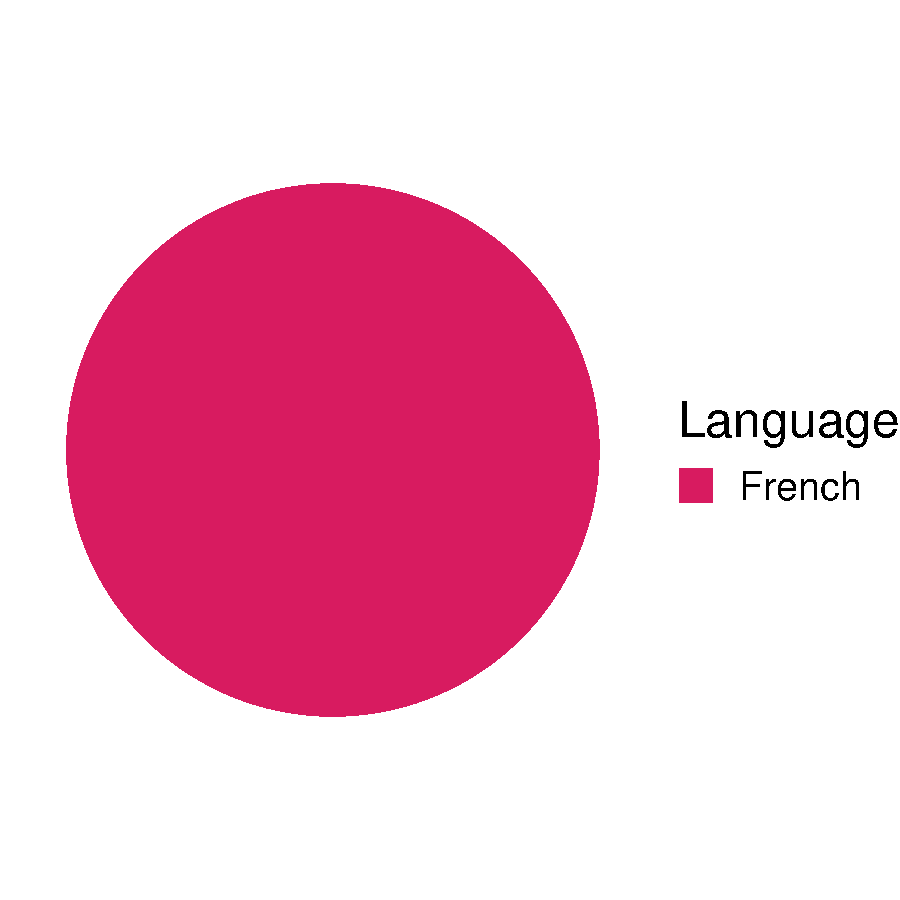
\includegraphics[width=\maxwidth]{figure/unnamed-chunk-1-1} 

                Community 1340 (smaller)
              \end{center}
            \column{0.25\textwidth}
              \begin{center}

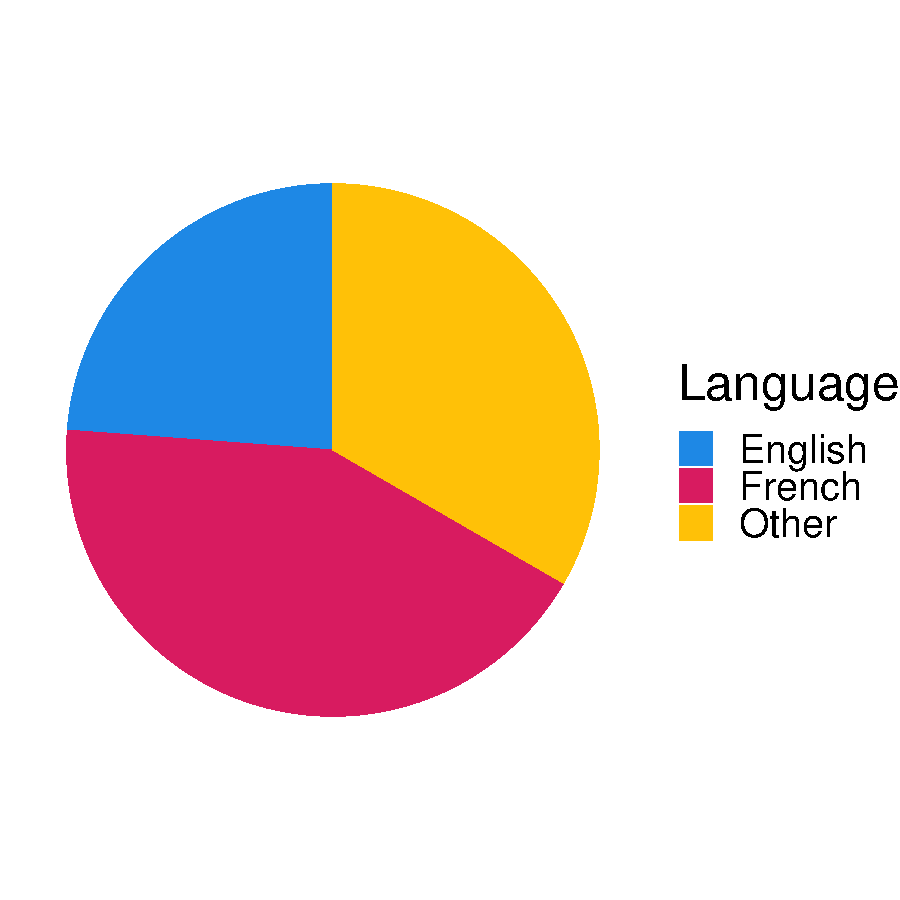
\includegraphics[width=\maxwidth]{figure/unnamed-chunk-2-1} 

                Community 6817 (bigger)
              \end{center}
            \column{0.25\textwidth}
              \begin{center}

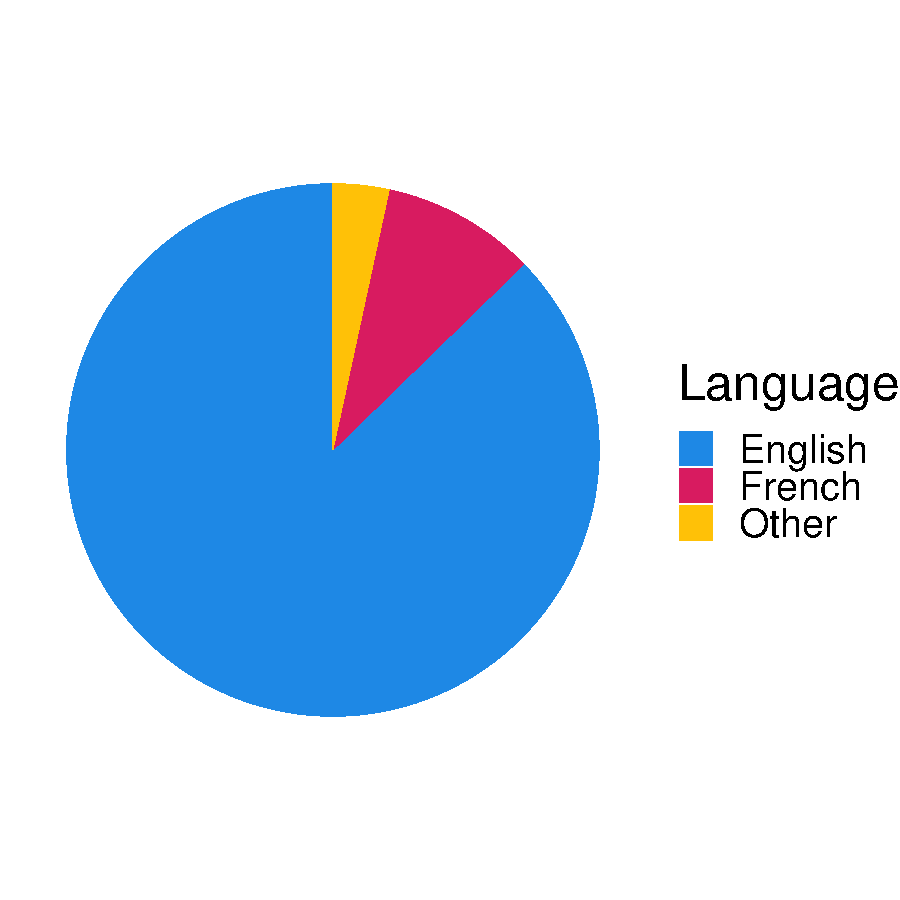
\includegraphics[width=\maxwidth]{figure/unnamed-chunk-3-1} 

                Community 1291 (bigger still)
              \end{center}
            \column{0.25\textwidth}
              \begin{center}

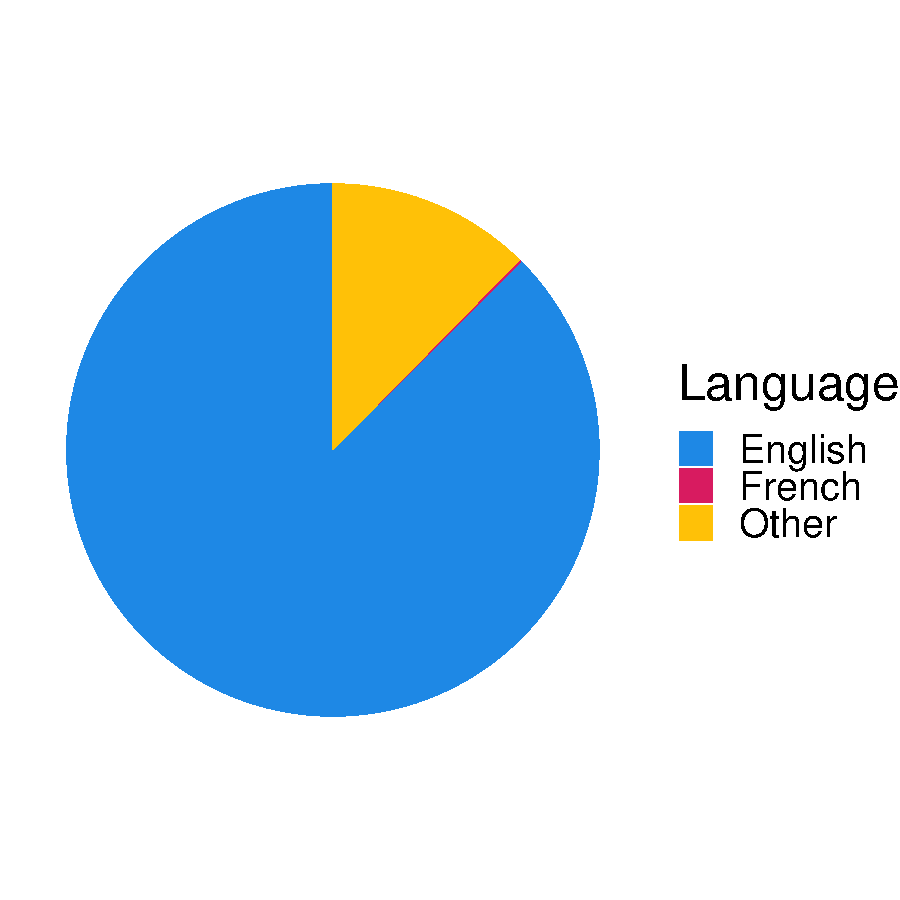
\includegraphics[width=\maxwidth]{figure/unnamed-chunk-4-1} 

                Community 1032 (biggest)
              \end{center}
          \end{columns}
        \end{block}

        \begin{columns}
          \column{0.4\textwidth}
            \begin{block}{The outlier}
              The only French user of (lol) in community 1340: \alert{In-degree = 0}, out-degree = 50
              \begin{center}
                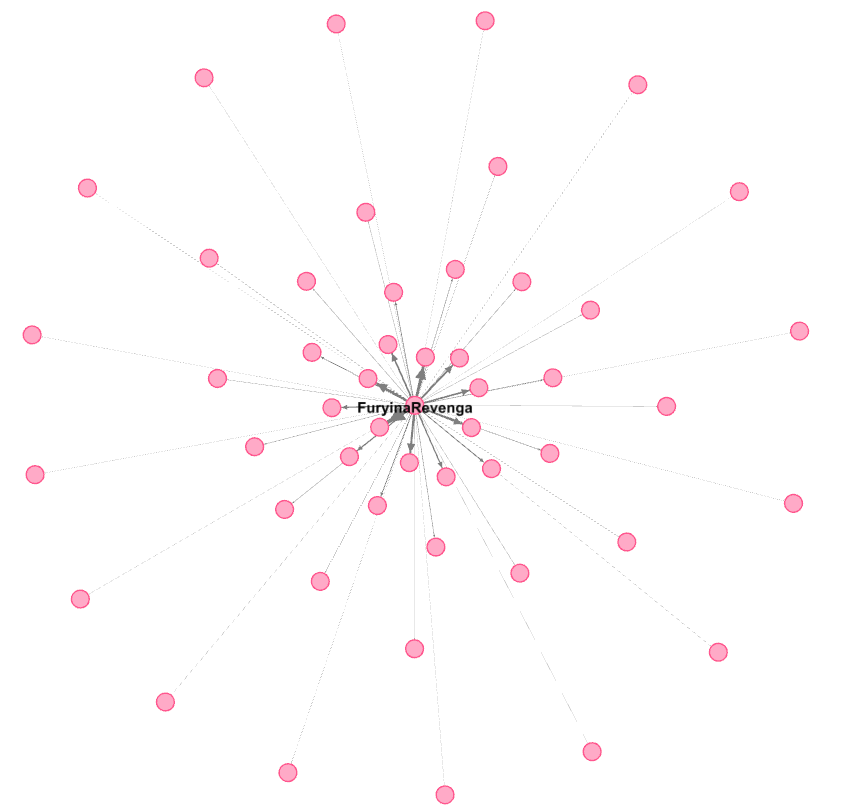
\includegraphics[scale=0.95]{ego_fury.png}
              \end{center}
            \end{block}
          \column{0.59\textwidth}
            \begin{block}{}
              There's a statistical relationship between community and province ($P < 0.0005$), though its far from exclusively one province per community

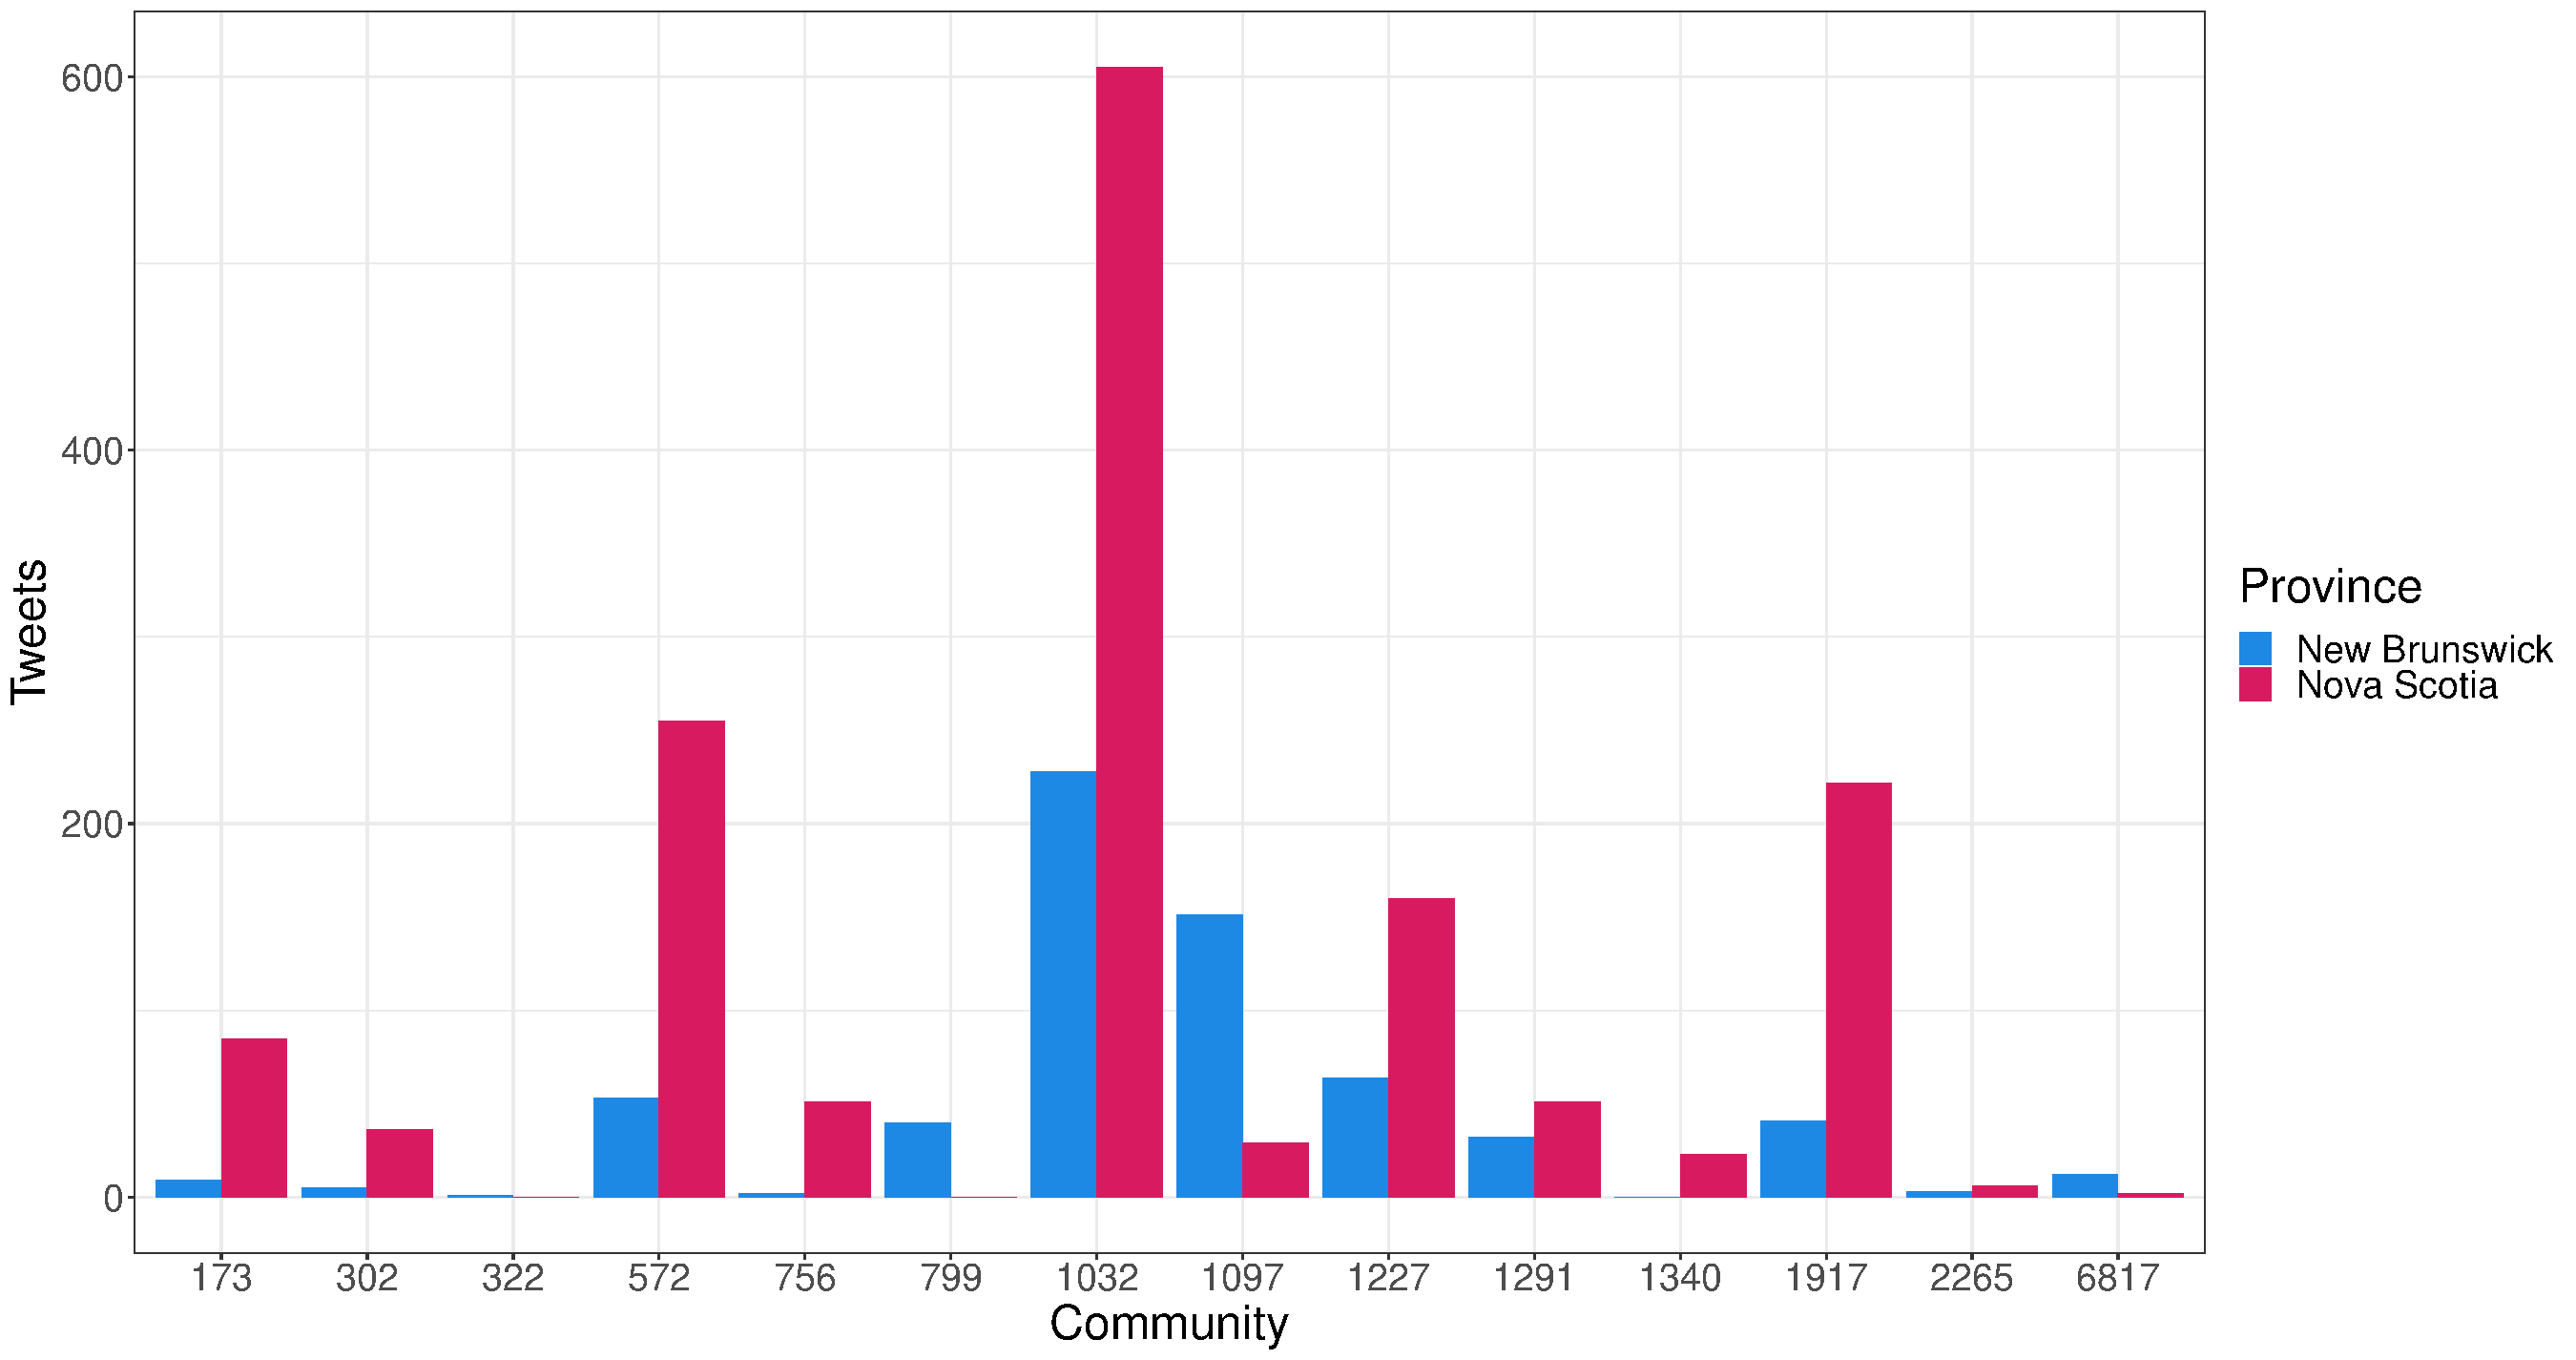
\includegraphics[width=\maxwidth]{figure/unnamed-chunk-5-1} 

            \end{block}
        \end{columns}

      %%%%%%%%%%%%%%%%%%%%%%%%%%%%%%%%
      % Right column (discussion)    %
      %%%%%%%%%%%%%%%%%%%%%%%%%%%%%%%%
      \column{0.19\textwidth}
        \begin{block}{Conclusion}
          The lexical variable (lol) as used in French tweets \emph{do} vary according to detected community
          \begin{itemize}
            \item The higher the presence of English, the more likely the use of the variant \lexi{lol}
          \end{itemize}
        \end{block}

        \begin{block}{Discussion}
          In online communities, French can be locally dominant but otherwise a minority, just as in geographical Maritime communities
          \begin{itemize}
            \item This appears to impact the way (lol) is used from community to community
          \end{itemize}
          Some users produce \emph{only} the variant \lexi{lol} in French tweets
          \begin{itemize}
            \item e.g., bloggercharles in the large, heavily English community 1097
            \item These users may not have \lexi{mdr} in their mental grammars
          \end{itemize}
          The methods used here highlight the importance of interactions more than other community concepts
          \begin{itemize}
            \item Detected communities are complementary to other concepts
            \item e.g., Detect communities first, then do an ethnography
          \end{itemize}
        \end{block}

        \begin{block}{References}
          \printbibliography
        \end{block}
    \end{columns}
  \end{frame}
\end{document}
